%%%%%%%%%%%%%%%%%%%%%%%%%%%%%%%%%%%%%%%%%%%%%%
%                insertmeeting
% 1) Title (something creative & funny?)
% 2) Date (MM/DD/YYYY)
% 3) Location (ex. Hagerty High School)
% 4) People/Committees Present 
% 5) Picture 
% 6) Start Time & Stop Time (ex. 12:30AM to 4:30PM)
%%%%%%%%%%%%%%%%%%%%%%%%%%%%%%%%%%%%%%%%%%%%%%
\insertmeeting 
	{Space Coast League Championship} 
	{02/06/22} 
	{Hagerty High School}
	{James, Jensen, Nathan, Ritam}
	{Images/RobotPics/robot.jpg}
	{9:30 - 6:30}
	
\hhscommittee{Software}
\noindent\hfil\rule{\textwidth}{.4pt}\hfil
\subsubsection*{Goals}
\begin{itemize}
    \item Compete at Leagues

\end{itemize} 

\noindent\hfil\rule{\textwidth}{.4pt}\hfil

\subsubsection*{Accomplishments}
Today was the League championships. In the morning our team competed in the qualification matches. Using all of the changes and fixes from the last month, our robot performed well. Our qualification scores, combined with our matches from the previous league meets, placed us as the first seed. We selected teams 7592 Roarbots and 4228 Gears of Other Dimensions as our alliance partners. We ended up playing two matches in the semifinals and three matches in the finals. The finals were played against our sister team 4227, putting a lot at stake for both teams. Our driveteam worked well with our alliance partner to perform well, leading to our alliance taking 1st place. After the matches concluded, our robotics program focused on cleaning up the fields, supplies, and concessions stand before Monday. Although our robot performed well, there were many changes we should focus on for the next month. 


\begin{figure}[htp]
\centering
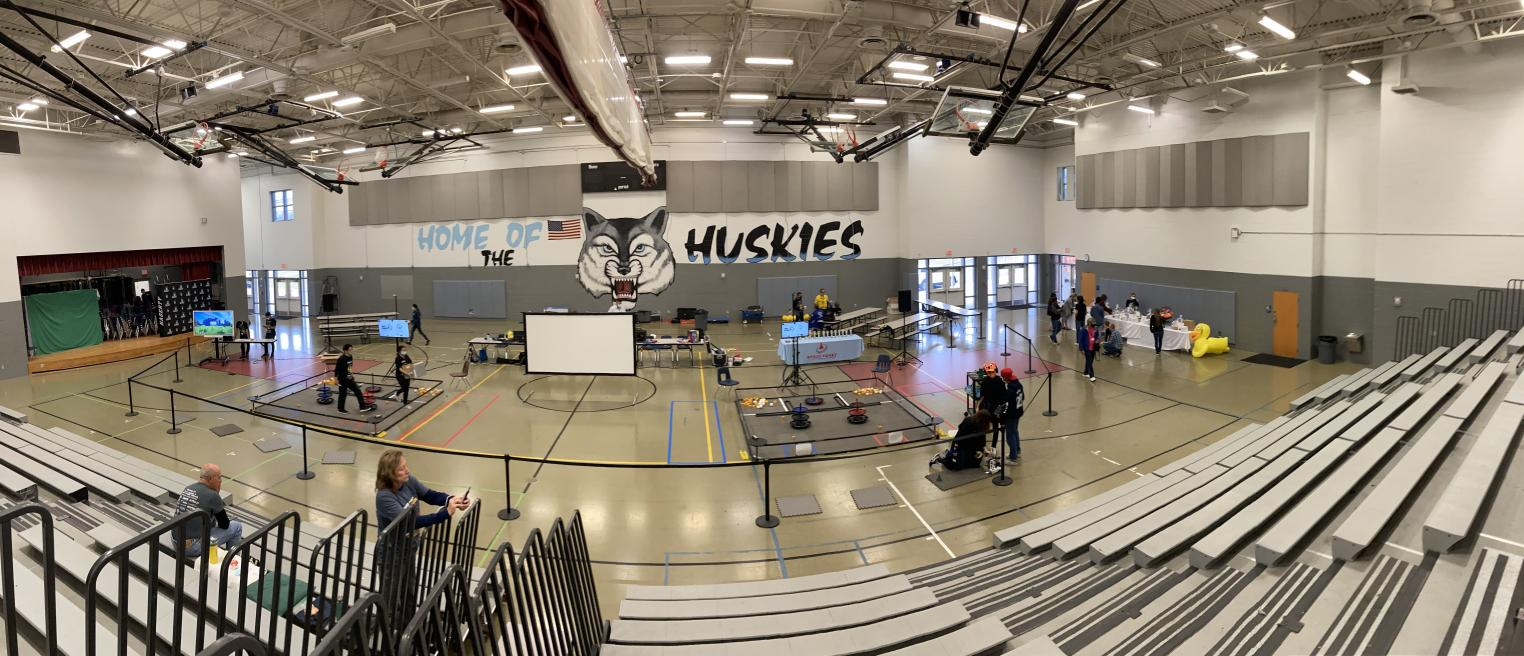
\includegraphics[width=0.95\textwidth, angle=0]{Meetings/February/02-06-22/02-06-22 1.jpg}
\caption{The gym used for the competition}
\label{fig:020622_1}
\end{figure}

\begin{figure}[htp]
\centering
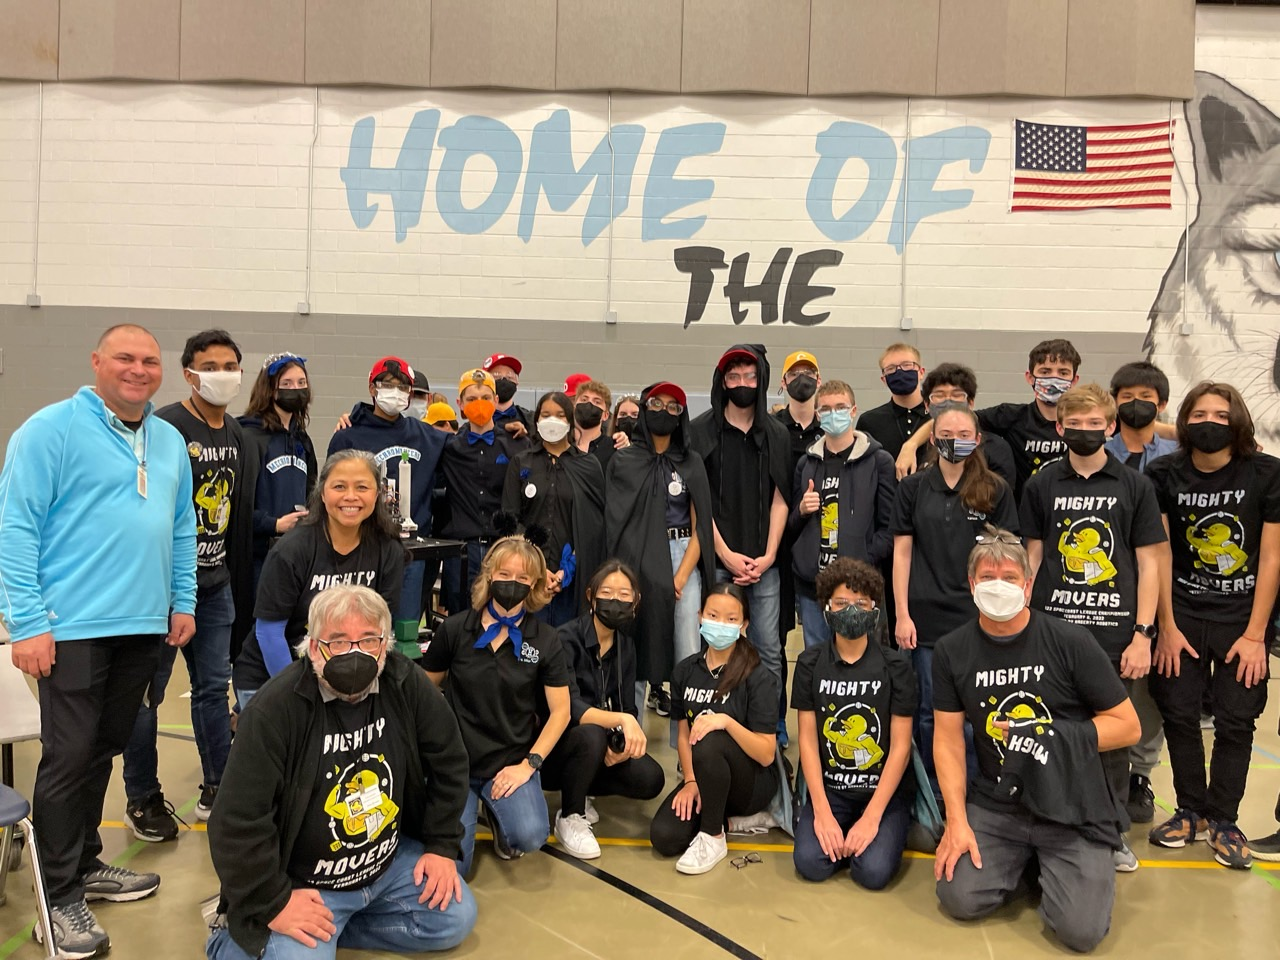
\includegraphics[width=0.95\textwidth, angle=0]{Meetings/February/02-06-22/02-06-22 2.jpg}
\caption{Hagerty Robotics FTC Teams 4717 and 4227}
\label{fig:020622_2}
\end{figure}


\whatsnext{
\begin{itemize}
    \item Plan a list of components to improve on the robot
    \item Refine our presentation and portfolio
    \item Create posters and update our spellbook for the next competition
\end{itemize} 
}

